\documentclass[a4paper,12pt]{article}
\usepackage[utf8]{inputenc}
\usepackage{setspace}
\usepackage{graphicx}
\usepackage{caption}
\usepackage{subcaption}
\usepackage{hyperref}


\title{CS 6161: Analysis of Algorithms\\
Report on Final Project -TSP Art}
\author{Saikat Chakraborty (sc2nf@virginia.edu)\\Tanmoy Sen (ts5xm@virginia.edu)}

\begin{document}
\date{}
\maketitle

%\doublespacing
\medskip

Algorithmic Art is a creative blend of programming, design, and the arts where the design is generated using an algorithm. Among the diverse forms of algorithmic arts, we have also implemented the TSP art as part of our term project for the course CS 6161.  

\medskip

\section{Project Specification}
TSP art or travelling salesman problem art, an art form invented by Robert Bosch, is an image which can be drawn with one single line. In essence, it is the art that will be generated if one draws it by hand he can use one single stroke without lifting his pencil. The goal of our project is to generate the TSP art given an image as input. Although most of the TSP art format are limited to monochrome image format, we have implemented the color formatted TSP art using a simple heuristic with a motive to generate the color illusion of the original image.    

\medskip

\section{Implementation Overview}
TSP art applies the concepts and heuristics of the Traveling Salesman Problem to the realm of the arts. As, an image can be considered a matrix of pixels, or tiny dots of color if we view these dots as the set of points in the traditional Traveling Salesman Problem, then we can apply TSP heuristics to an image. The high-level process we followed in our implementation is as follows: we take an image, create a “stippled” or dotted version of the image, and then connect the dots using a TSP heuristic. The resulting image is one long, uninterrupted line that connects all the dots.

\medskip

 
\section{Implementation Details}
While implementing the TSP art program, we have followed an iterative process using step-wise heuristics to gradually build the program. The steps during the implementation are as follows:
\begin{itemize}
    \item Generation of stippled image
    \item Implementation of the TSP heuristics
    \item Swapping the Lines for improved image
\end{itemize}

This section describes the in-depth processing of each steps. Figure 1 summarizes the output after running each of the processes on the input image.  


\subsection{Generation of stippled image}
For the generation of the stippled image, we first convert the input image to monochrome and gather the pixel information of the image. Then to accomplish the generation step, we constructed a grid from the image, where each cell in the grid is a certain dimension,  To accomplish this step, I constructed a grid from the image, where each cell in the grid is a certain dimension, such as 3x3, 4x4, 5x5, etc. The dimension of the grid is set by the user at the beginning of running the program.  Each of these cells holds a single pixel to represent all the pixels in that particular cell.  The single pixel’s color is the average color of all the pixels in that region. This pixel will be represented as a node in the graph while running the TSP heuristics. But, the existence of a node in a particular cell is defined if the average of that cell exceeds a certain threshold limit of the overall mean of that image. The threshold limit is defined by multiplying the average value of that particular cell by a parameter $\alpha$, where $0<\alpha \leq1$. The value of the $\alpha$ is also set as an user input. We have placed the pixel(node ) in a random location in the block to ensure generation of a more stippled image. 

\begin{figure}[htb]
\centering
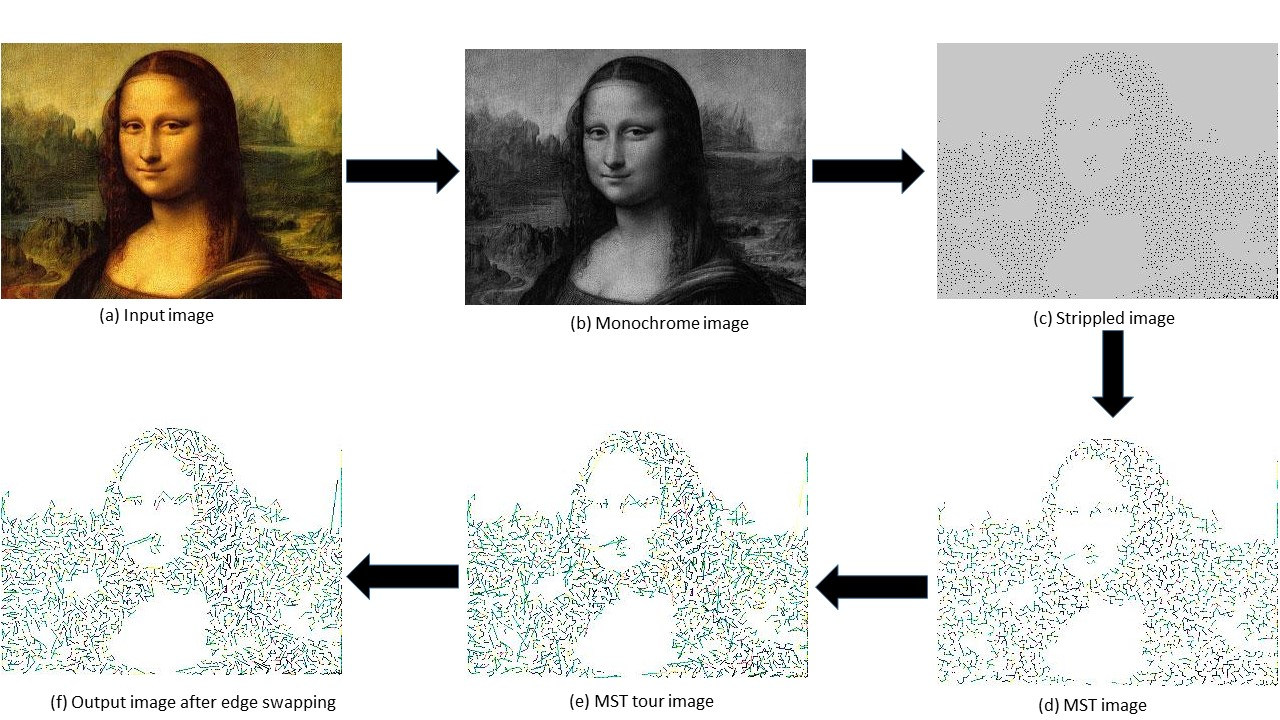
\includegraphics[width=\textwidth]{Report.jpg}
\caption{Output Generated after execution of each process}
\label{fig:pc3}
\end{figure}


\subsection{Implementation of the TSP heuristics}
After generating the stippled image, the next step is to connect the dotted lines using a TSP heuristics. In order to accomplish this, we have first formed a complete graph of the nodes(pixels) generated the process mentioned in the previous subsection where the distance between the nodes are euclidean distance between the pixels in the input image. On the complete graph, Kruskal Algorithm is being run in order to find the minimum spanning tree. In addition to being the part of the TSP heuristics, it gave us which produces a different artistic appearance. Next, we have formed the TSP tour out of the tree generated at the previous step. At this stage of our implementation, it seems  some intersecting lines are being drawn across the image.

\subsection{Swapping the Lines}
In order to improve the images, we have implemented a 2-Opt heuristic. 2-Opt improves an existing TSP tour by swapping certain edges if the resulting path creates a shorter tour. First, we detect whether there is any intersections  lines. If we find any intersections, the source and destination of the lines are interchanged as such there is no intersection between the lines. In addition, we also reverse the direction of the edges that were found non-intersecting up-to those intersecting images. This process is repeated until no intersecting lines are detected. But, this process can run for a long period of time. In order to shorten the period, we have kept a provision for user to define how many iterations he wants the swapping process to run. Ultimately,  this results in a shorter overall tour, as well as an improved version of TSP art.

\medskip
\section{Inputs and Outputs}
We have created a graphical user interface to accommodate the inputs taken from the user. The  main inputs that are taken from the users are, $\alpha$, block size and the number of iterations of the 2-opt heuristics that were mentioned in the previous subsections. Along side these three inputs, a separate input scale is taken, in order to magnify the output images to the level defined by the users. Figure 2 demonstrates the user interface that is designed to take the inputs. As output, we generate three images, the MST image, the tour image and finally the TSP art image. While generation of the color images, the lines are drawn from source node's color code value to destination node's color code maintaining gradual increase as followed in gradient line drawing. We have also kept a provision of storing the images on black background or night mode version so that the color lines are more visible. Figure 3 shows the drawings on black background of the corresponding images. In the graphical interface we have also kept the provision of saving them as necessary.

\begin{figure}[htb]
\centering
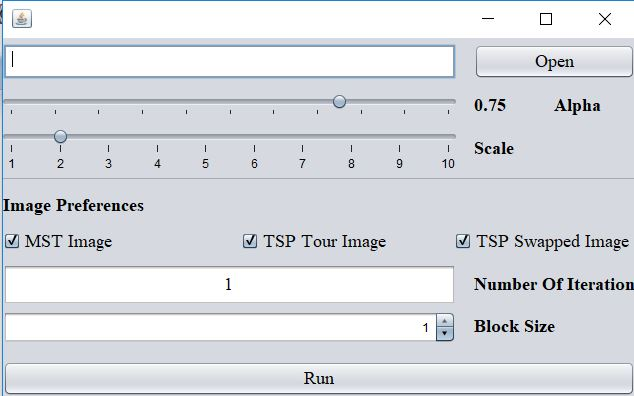
\includegraphics[width=0.6\textwidth]{Capture_GUI.JPG}
\caption{Graphical User Interface}
\label{fig:pc2}
\end{figure}


\begin{figure}[htb]
\centering
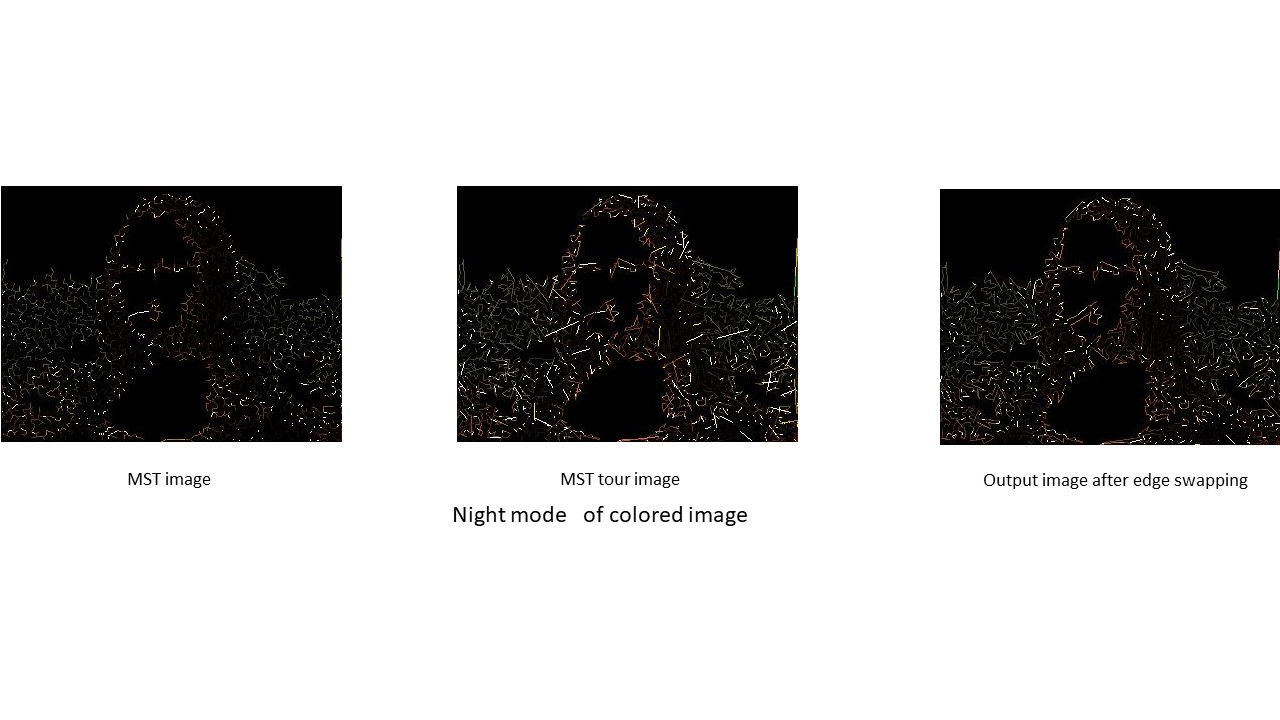
\includegraphics[width=\textwidth]{Presentation2.jpg}
\caption{Output generated on black background}
\label{fig:pc}
\end{figure}

\medskip

\section{Order of the Implementation Processes}
Generation of the stippled image is part of the pre-processing of the TSP art drawing, consequently, we do not consider its execution time in our consideration. Table 1 summarizes the order of other processing steps.

\begin{table}[h!]
\label{table:summary}
\caption{Order of the Algorithms}
\begin{tabular}{ |p{3.5cm}||p{3.5cm}|p{3.5cm}|}
 \hline
 \multicolumn{3}{|c|}{Processes and their order of execution} \\
 \hline
 Process & Order & Symbols \\
 \hline
 MST	& $O(|E|log|V|)$ & $E$ and $V$ is the number of edges and nodes in the generated complete graph from the stippled image\\
 \hline
 MST Tour & $O(|V|)$ &  $V$ is the number of nodes in the MST\\
 \hline
 2-opt heuristics & $O(k.|V|^2)$ & $k$ is the number of iterations and $V$ is the number of vertices in the MST tour\\
 \hline
 \end{tabular}
 \end{table}
\medskip

\section{Language and Library Used}
We have implemented the program using java.  we have used the opencv library for converting  the input image to monochrome. 

\section{Problems Encountered}
Initially, we have faced some issues regarding the run time of our implemented minimum spanning tree using kruskal algorithm. The implementation used to take a huge amount of time to generate the MST. Then we updated our data structure and used the set class in java which decreased the run-time significantly. Moreover, the swapping of edges can run indefinitely, so in order to finish the run, we added a user-defined parameter to set the iteration of swapping process. 

\medskip
\section{Conclusion} 
In this report, we present the process of implementing TSP art using our heuristics. During the implementation we learned the importance of algorithm analysis and choosing the best algorithm for the situation.  For this particular application, we think longer run-time is worthwhile because the resulting images are so much more pleasing. 

\medskip
\section{Code URL}

\url{https://github.com/Tanmoy058/TSP-Art/tree/master/src/edu/virginia/cs/tspim}

%\bibliographystyle{unsrt}%Used BibTeX style is unsrt
%\bibliography{sample}

\end{document}
